\documentclass[conference]{IEEEtran}
\IEEEoverridecommandlockouts
% The preceding line is only needed to identify funding in the first footnote. If that is unneeded, please comment it out.
\usepackage{cite}
\usepackage{amsmath,amssymb,amsfonts}
\usepackage{algorithmic}
\usepackage{graphicx}
\usepackage{textcomp}
\usepackage{xcolor}
\def\BibTeX{{\rm B\kern-.05em{\sc i\kern-.025em b}\kern-.08em
    T\kern-.1667em\lower.7ex\hbox{E}\kern-.125emX}}
\begin{document}

\title{Dealing with Imbalance in Computer Vision\\}

\author{\IEEEauthorblockN{Ashok Meyyappan}
\IEEEauthorblockA{\textit{CSCE 421 Final Project} \\
\textit{November 23, 2020}\\}
}

\maketitle

\begin{abstract}
    In this report, I present the current problems of image recognition and imbalance issues. To analyze the problems, I introduce the imbalanced datasets that will help in handling data imbalance. Following the understanding of the problem and introduction of the datasets, I discuss the models I utilize to handle data imbalance and their respective accuracy. I dive into the differences between the models, such as their features and implementation details. To analyze the effectiveness of the models, I describe and explain the testing results, and how they differ. Following analysis and discussion, I provide my overarching observations regarding the issues of imbalance and the models I created. 
\end{abstract}

\section{Introduction}
Image recognition is similar to computer vision, but not exactly the same. It is about the pixel and pattern analysis of an image to recognize the image as a particular object rather than the ability to do something with the recognized images. The process of image recognition is to first extract pixels features from the image, and then prepare labeled images for training the model. Once the images are prepared, the training is then accomplished to categorize the images. An unknown image is then predicted to be a part of one of the categories, which also goes through the pixel feature extraction process [3]. 

In image recognition, there exists class imbalance issues. Class imbalance occurs when rare events are analyzed, as the number of normal samples is generally much greater than the occurrence of abnormal cases. Due to the rare nature of abnormal cases under analysis, the amount of available samples for the abnormal cases is generally small, but the information associated with each case can be significant. Consequently, the ratio of the samples per class to the available features per sample may cause biased categorization results [2]. There are other imbalances, such as spatial imbalance and scale imbalance, but this paper focuses on the class imbalance within image recognition [1].

The situation of class imbalance can be worsened further in multi-class problems. The ratio of training instances among different classes can drastically differ. However, it can be coarsely categorized in two specific types of imbalance, i.e. step imbalance and linear imbalance [4].

In step imbalance, within majority classes and minority classes the instances are roughly the same, but the difference between them majority and minority can be large. In linear imbalance, the different classes have different instances but the number can be coarsely interpolated linearly from smallest class to biggest class. The algorithm takes these two datasets to create the models that handle the data imbalance and evaluates its accuracy with the AUROC metric. 

\section{Method Differences}
The methods that were implemented were the logistic regression model, random forest model, and the convolutional neural network (CNN) technique. Prior to implementation of all the methods, the training and testing datasets are loaded and generate dataloaders with a batch size of 64 for the training sets and a batch size of 1000 for the testing set. It is important to note that the same process was implemented for both the step and linear training sets when creating a model for each imbalance per method.

\subsection{Logistic Regression}
The logistic regression model is a linear model that models the probability of the default class or the first class. Though this is classified as a linear model, the predictions are transformed using the logistic function:  
\begin{equation}
\frac{1}{1 + e^{-x}}\label{eq}
\end{equation}
An S-shaped curve is formed from Eq. (1), which can take any real-valued number and map it into a value between 0 and 1 [13]. As a result, the 0 value was set to 0, while the rest was set to 1 for the labels of both the training and testing set. 

Since these models were not created with PyTorch, the dataloaders were flattened into lists through a double for loop. The flattened data was reshaped when split into X and y, or features and labels respectively. 

Logistic regression with a stratified k-fold cross validation was preformed on the training sets. This particular method was implemented rather than random sampling, so that the entire training sets would be represented in equal proportions with precision [10]. Stratified sampling was preformed with a 10-fold cross validation to partition the training sets into 10 equally sized sub-samples. 10 was the best option for k in this model primarily based on the fact that higher k values are preferred for larger sample sizes. The logistic regression that was performed within the stratified k-fold cross validation had a maximum iteration of 100000000 and a penalty of 'l2'. An L2 regularization was included to deal with the multi-class nature of the problem. 

Following the completion of the train and test splits of the training sets within the stratified k-fold cross validation, the training and testing features were standardized to make the features look like standard normally distributed data [12]. 

A normal logistic regression model was then performed on the overall training set and a prediction was found for testing purposes. This was done after the stratified k-fold cross validation to improve the accuracy of the models by further training the training sets. The logistic regression model had a C parameter of 0.01, maximum iteration of 100000000, and solver as 'lbfgs'. The C parameter is basically the regularization parameter of the models, in which the formula is C = $\frac{1}{\lambda}$. A low 0.01 C value was chosen to increase the regularization strength [11]. 

\subsection{Random Forest}
The random forest model is a higher-order model that builds multiple decision trees and merges them together, and can be used for both classification and regression problems [7]. The manual feature extraction techniques for this model are entropy and gini index. 

Since these models were not created with PyTorch like the logistic regression models, the dataloaders were flattened into lists through a double for loop. The flattened data was reshaped when split into X and y, or features and labels respectively. 

The random forest model has a regressor and a classifier. Regression involves dealing with continuous values and the mapping of values to continuous output. On the other hand, classification involves dealing with discrete values and the mapping of values to predefined classes [14]. The random forest classifier (fr\_classifier) was chosen for these models because this is a binary classification problem. 

As mentioned earlier, the manual feature extraction techniques for the random forest model are entropy and gini index. Gini index measures the total variance across K classes, as shown in this equation: 
\begin{equation}
G = \sum_{k=1}^{K} p_{mk}(1 - p_{mk})\label{eq}
\end{equation}
In comparison, entropy takes a value near 0 if all the p are near 0 or 1, as shown in this equation: 
\begin{equation}
H = -\sum_{k=1}^{K} p_{mk}log(p_{mk})\label{eq}
\end{equation}
Taking into account the purpose of both criterion and the higher accuracy for entropy during testing, entropy was used for these models. The maximum depth was found following the testing of maximum depths ranged from 1-10, in which 10 had the highest accuracy. 

The maximum depth, criterion, and random forest type were the parameters to the 'cross\_validate\_args()' function alongside the features and labels of the training sets. This function calls both the 'cross\_validate\_models()' and the 'name\_creator()' functions. The 'name\_creator()' function creates a string name for each depth value with respect to the number of folds and criterion. The 'cross\_validate\_models()' function calls the 'cross\_validate\_single\_model()' function. This function performs a stratified k-fold based on the number of folds and a train-test-split. In this case, it would perform these on the training sets. The respective model's function would be called from the sklearn library, which would be the random forest classifier function in this case. 

Following the completion of the random forest classifier with stratified k-fold on the training sets, the general random forest classifier function was invoked and a prediction was found for testing purposes. The parameters consisted of the default 10 estimators or the number of trees, and a random state of 1 to limit the randomness of the bootstrapping. 

\subsection{Convolutional Neural Network}
The CNNs is similar to Neural Networks, in which they are made up of neurons that have learnable weights and biases. CNNs perform a dot product and make the assumption that the inputs are images [9]. 

Since these models were created with PyTorch, there was no need to flatten or reshape the dataloaders of the imbalanced datasets. 

A simple CNN architecture is utilized, which consists of 2 convolutional layers for feature extraction from images [15]. The forward method or pass in the CNN class is the mapping that maps an input tensor to a prediction output tensor [16]. The architecture of the model results in two convolutional layers and two linear layers, in addition to two dropouts for regularization. The linear layer was calculated as shown: 
\begin{equation}
\frac{I - K + 2P}{S} + 1, \label{eq}
\end{equation}
where I is neuron size, K is kernel size, P is padding, and S is stride. The forward method additionally consists of the Rectified Linear Unit or ReLU for the increase of non-linearity in the images [17].

Following the creation of the CNN architecture, a classification cross-entropy loss and SGD with learning rate is used to measure the probability of the model with outputs between 0 and 1, and to control the quickness of adaptation to this problem. The models are trained by first looping through the dataset. Within the for loop, the images and labels iterate through the training dataloader, continuously feeding inputs to the network and optimizing. The test dataloader is looped through as well, but will be further discussed in the test results section. 

\subsection{Summary}
As can be seen, there were major differences between the implementation of all three methods for the imbalanced linear and step datasets. The random forest and logistic regression models were most closely related of the three, in that both performed stratified k-fold and train-test-splits on the training sets. Both varied based on the concept of one involved regression and the other involved classification. The CNN method was slightly varied from the two due to how the dataloaders were not flattened and PyTorch was utilized to aid in creating the models. 

\section{Test Results}

After the creation and during the creation of the models, the models were tested on both the testing set split from the training set and the actual testing test. The method of testing utilized for logistic regression model, random forest model, and the CNN technique was intended to determine the accuracy or AUROC score. For the multi-class parameter, 'ovr' or one-vs-the-rest was used to allow binary classification algorithms for multi-class classification. It is important to note that these steps are crucial in determining whether the implementation needed any changes to perfect the existing models.  

\subsection{Logistic Regression}
The logistic regression model creation process consisted of two primary testing steps. The first was involved with the training set and the second was involved with actually testing for the models' AUROC scores. 

The first accuracy test was with the training set within the stratified k-fold cross validation implementation. The prediction value used for determining the AUROC score was the testing set from the overall training set. The AUROC score was determined by dividing the score calculated from the 'roc\_auc\_score()' function by the number of folds to get the score of the specific portion. The AUROC score was greater than 90\%, which was the signal to move on to the next step of the logistic model creation process. 

The second accuracy test was the actual testing phase to get the final AUROC score. Prior to the prediction step, the features of the testing set was changed to a binary form by setting anything that equals 0 as 0, and the rest as 1. The AUROC score generated for the imbalanced step dataset was approximately 0.998057. The AUROC score generated for the imbalanced linear dataset was approximately 0.998072. 

\begin{figure}[htbp]
\centerline{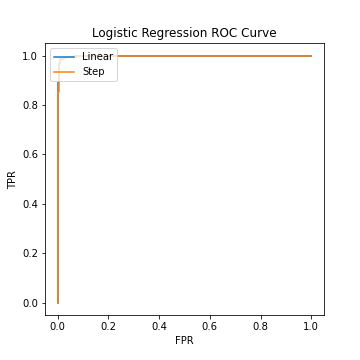
\includegraphics[width=0.9\columnwidth]{logreg_linear_step_roc_curve.png}}
\caption{ROC Curve Logistic Regression}
\label{fig}
\end{figure}

Some interpretations can be made based on the AUROC scores. Both the imbalanced linear and step datasets have approximately the same rounded AUROC score. This may happen due to the stratified k-fold cross validation utilized on the training sets to keep the precision. The slightly lower AUROC score for the imbalanced step dataset can be understood by the majority and minority class concept.   

\subsection{Random Forest}
The random forest model creation process consisted of two primary testing steps like the logistic regression models. The first was involved with the training set and the second was involved with actually testing for the models' AUROC scores.

The first accuracy test was with the training set within the cross validation functions and stratified k-fold implementation. There two specific parts to this accuracy test. One was to determine the maximum depth that would be used for the final model. By collecting the AUROC scores for a range of maximum depths that were both above and below 90\%, it was determined that the maximum depth of 10 was the most accurate. The second part of this test was to determine whether the precision of the stratified k-fold actually happened by running the maximum depth of 10 again. As expected, the AUROC score was around the exact same as before.

The second accuracy test was the actual testing phase to get the final AUROC score. Prior to the prediction step, the features of the testing set was changed to a binary form by setting anything that equals 0 as 0, and the rest as 1. As noticed, this step of the process is exactly the same as for the logistic regression testing. The AUROC score generated for the imbalanced step dataset was approximately 0.998630. The AUROC score generated for the imbalanced linear dataset was approximately 0.999189.

\begin{figure}[htbp]
\centerline{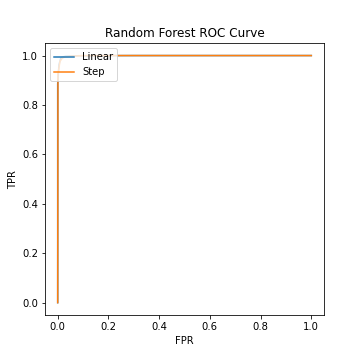
\includegraphics[width=0.9\columnwidth]{rf_linear_step_roc_curve.png}}
\caption{ROC Curve Random Forest}
\label{fig}
\end{figure}

Some similar interpretations to the logistic regression testing results can be made based on the AUROC scores. Both the imbalanced linear and step datasets have approximately the same rounded AUROC score. This may happen due to the stratified k-fold cross validation utilized on the training sets to keep the precision. The slightly lower AUROC score for the imbalanced step dataset can be understood by the majority and minority class concept. 

\subsection{Convolutional Neural Network}
The CNN model creation process consisted of three primary testing steps. The first was involved with the accuracy based on iterations. The second was involved with the accuracy on 1000 images. The third was involved with the actually testing for the models' average AUROC score. 

The first accuracy test was with iterations during the model training process. As the optimizations were taking place and the values were being sent to the network, the count of correctly predicted images from looping through the test dataloader was utilized to calculate an accuracy percentage [6]. The number of epochs used to perform the for loop for training the model was set to 3, since previous testing determined there was no or limited change following the third epoch. The results of this test for the imbalanced step dataset can be seen here:
\begin{itemize}
  \item Iteration: 500. Accuracy: 84
  \item Iteration: 1000. Accuracy: 89
  \item Iteration: 1500. Accuracy: 92
\end{itemize}
The results of this test for the imbalanced linear dataset can be seen here:
\begin{itemize}
  \item Iteration: 500. Accuracy: 77
  \item Iteration: 1000. Accuracy: 86
  \item Iteration: 1500. Accuracy: 90
\end{itemize}
As can be seen in the results, the accuracy crosses or is at 90\% for both, indicating an accurate model so far. The increase in accuracy in relation to the increase in iterations can be interpreted as due to the amount of time the model has to run or iterate through the datasets.

The second accuracy test evaluated the model for its accuracy on 1000 images. The model is under model evaluation mode for this test portion, which disables any batch normalization layers. Prior to testing, the autograd functionality is disabled to speed up computation from reducing unnecessary waste. The accuracy steps being preformed is similar to the testing step during the training of the model, except this only iterates through the test dataloader [4]. The accuracy on 1000 images resulted in 96.98\% for the imbalanced step dataset and 95.37\% for the imbalanced linear dataset. 
\begin{figure}[htbp]
\centerline{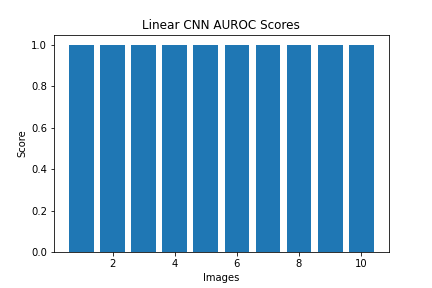
\includegraphics[width=0.6\columnwidth]{auroc_linear_cnn.png}}
\caption{Linear CNN AUROC Scores}
\label{fig}
\end{figure}
This high percentage additionally confirms the accuracy of the models. The high accuracy percentage can be interpreted as the result of specific layer inputs. 

The third accuracy test was the actual testing phase of these models. The AUROC scores were calculated by appending AUROC scores within the iteration utilized to achieve the second accuracy test. With the assistance of Softmax and the multi-class parameter 'ovr', the average AUROC score was calculated for both datasets. The imbalanced step dataset achieved an average AUROC of approximately 0.999378 and the imbalanced linear dataset achieved an average AUROC of approximately 0.998581. The similarity between the rounded AUROC values for both the step and linear imbalanced datasets can be interpreted to be because of the high amount of iterations. The slightly lower AUROC for the imbalanced linear dataset can be interpreted to be because of the different instances per class within the train and test loaders. 

\subsection{Summary}
Similarities and differences can be seen from each accuracy and all the AUROC scores for each model and both imbalanced datasets. Though the AUROC scores remained really close, the slight comparisons between the imbalanced linear dataset and the imbalanced step dataset were shown and explained. 

\section{Comparison of Techniques}

To comprehend the analysis and comparison of techniques and results, it is vital to understand what exactly AUROC means. AUROC stands for Area Under the Receiver Operating Characteristics. The reason why AUROC is primarily utilized as the evaluation metric is because the traditional metric may be biased to the majority class. AUROC's primary purpose is to check a classification model's performance. 

Prior to comparing the techniques' results, the overall results across the techniques will first be displayed and can also be viewed in the testing results section for initial interpretations. 
\begin{itemize}
    \item Logistic Regression (Linear): 0.998072
    \item Logistic Regression (Step): 0.998057
    \item Random Forest Classifier with Entropy (Linear): 0.999189
    \item Random Forest Classifier with Entropy (Step): 0.998630
    \item CNN (Linear): 0.998581
    \item CNN (Step): 0.999378
\end{itemize}
As can be seen by the results, all three techniques had a rounded AUROC score of 0.99. These scores are really similar for the logistic regression and random forest models due to the stratified k-fold that is performed on the training test. 

Looking more closely in detail at the logistic regression and random forest AUROC scores, the random forest scores are slightly higher. This is due to the classification aspect of the problem rather than the dealing of continuous values involved in regression models. It may also be due to the fact of logistic regression's limitation to one probability statement compared. Due to random forest consisting of many trees with various levels of maximum depth, the random forest score appears slightly better than the logistic regression for the vast options. For instance, some maximum depths of random forest result were less than the logistic regression AUROC score.

Looking more closely in detail at the logistic regression and CNN AUROC scores, the CNN score tend to be higher. This is due to the lack of flattening and reshaping of the dataset, since the dataloader is directly inserted into the CNN model. It is also because of the large amount of iterations that takes place in the CNN models compared to the logistic regression models. This is highly evident in the much higher running time for CNN models.  

Looking more closely in detail at the random forest and CNN AUROC scores, there is no evident trend in scores as the imbalanced linear dataset is more accurate in random forest. In comparison, the imbalanced step dataset is more accurate in the CNN model. The imbalanced linear dataset is more accurate in the random forest model because the linear interpolation of smallest to biggest class is better accustomed to the random forest model. The imbalanced step dataset is more accurate  CNN model because the difference between the majority and minority class is less likely to be different in the CNN model. 


\section{Conclusion}
Due to the high AUROC scores for all the models, it is determined the effectiveness of the stratified k-fold and the increase in iterations. There are minimal differences in the numerical values of the AUROC results, despite each implementation varying largely per model. The precision of the AUROC scores following multiple re-runs of the program demonstrate that accuracy is not the models' only benefit. 

I improved my understanding of the logistic regression, random forest, and CNN methods, since comparing the really close results led to a deep analysis of the details of each method. I learned about the imbalance issues involved in image recognition, specifically step and linear imbalances. I learned various ways to approach machine learning problems, since the goal of this report was to approach this problem from three different methods. I learned of various ways to improve accuracy of models through trial and error, and research. Comparing the models and methods helped determine which methods are better suited for which situations. Lastly, I learned how to utilize PyTorch in terms of performing machine learning algorithms and models.

In the future, I hope to utilize what I've learned to possibly work on personal machine learning projects. Additionally, I may experiment more with this project to see how other models I did not use would perform. I also hope to utilize what I've learned with PyTorch and the various methods to potentially forecast important data and statistics. Working on this project and report has been a great learning and problem-solving experience, and enhanced my research abilities.  

\begin{thebibliography}{00}
\bibitem{b1} K. Oksuz, B. C. Cam, S. Kalkan, and E. Akbas, ''Imbalance Problems in Object Detection: A Review,'' March 2020.
\bibitem{b2} A. V. Sousa, A. M. Mendonça, A. Campilho, ''Image Analysis and Recognition,'' September 2006.
\bibitem{b3} ''What Is Image Recognition?'' November 2018.
\bibitem{b4} ''Convolutional Neural Networks Tutorial in PyTorch,'' April 2018.
\bibitem{b5} ''PyTorch Examples,'' unpublished.
\bibitem{b6} ''TRAINING A CLASSIFIER,'' 2017.
\bibitem{b7} N. Donges, ''A COMPLETE GUIDE TO THE RANDOM FOREST ALGORITHM,'' September 2020.
\bibitem{b8} ''Gini Impurity and Entropy in Decision Tree – ML,'' unpublished.
\bibitem{b9} ''CS231n Convolutional Neural Networks for Visual Recognition,'' unpublished.
\bibitem{b10} ''Stratified K Fold Cross Validation'', unpublished.
\bibitem{b11} I. Species, ''Tuning parameters for logistic regression,'' 2016.
\bibitem{b12} ''scikit-learn,'' unpublished.
\bibitem{b13} J. Brownlee, ''Logistic Regression for Machine Learning,'' August 2020.
\bibitem{b14} ''ML | Classification vs Regression,'' February 2019.
\bibitem{b15} P. Sharma, ''Build an Image Classification Model using Convolutional Neural Networks in PyTorch,'' October 2019.
\bibitem{b16} ''Neural Network Programming - Deep Learning with PyTorch,'' unpublished.
\bibitem{b17} ''Convolutional Neural Networks (CNN): Step 1(b) - ReLU Layer,'' August 2018.
\end{thebibliography}
\vspace{12pt}

\end{document}


